\documentclass{article}\usepackage{graphicx, color}
%% maxwidth is the original width if it is less than linewidth
%% otherwise use linewidth (to make sure the graphics do not exceed the margin)
\makeatletter
\def\maxwidth{ %
  \ifdim\Gin@nat@width>\linewidth
    \linewidth
  \else
    \Gin@nat@width
  \fi
}
\makeatother

\IfFileExists{upquote.sty}{\usepackage{upquote}}{}
\definecolor{fgcolor}{rgb}{0.2, 0.2, 0.2}
\newcommand{\hlnumber}[1]{\textcolor[rgb]{0,0,0}{#1}}%
\newcommand{\hlfunctioncall}[1]{\textcolor[rgb]{0.501960784313725,0,0.329411764705882}{\textbf{#1}}}%
\newcommand{\hlstring}[1]{\textcolor[rgb]{0.6,0.6,1}{#1}}%
\newcommand{\hlkeyword}[1]{\textcolor[rgb]{0,0,0}{\textbf{#1}}}%
\newcommand{\hlargument}[1]{\textcolor[rgb]{0.690196078431373,0.250980392156863,0.0196078431372549}{#1}}%
\newcommand{\hlcomment}[1]{\textcolor[rgb]{0.180392156862745,0.6,0.341176470588235}{#1}}%
\newcommand{\hlroxygencomment}[1]{\textcolor[rgb]{0.43921568627451,0.47843137254902,0.701960784313725}{#1}}%
\newcommand{\hlformalargs}[1]{\textcolor[rgb]{0.690196078431373,0.250980392156863,0.0196078431372549}{#1}}%
\newcommand{\hleqformalargs}[1]{\textcolor[rgb]{0.690196078431373,0.250980392156863,0.0196078431372549}{#1}}%
\newcommand{\hlassignement}[1]{\textcolor[rgb]{0,0,0}{\textbf{#1}}}%
\newcommand{\hlpackage}[1]{\textcolor[rgb]{0.588235294117647,0.709803921568627,0.145098039215686}{#1}}%
\newcommand{\hlslot}[1]{\textit{#1}}%
\newcommand{\hlsymbol}[1]{\textcolor[rgb]{0,0,0}{#1}}%
\newcommand{\hlprompt}[1]{\textcolor[rgb]{0.2,0.2,0.2}{#1}}%

\usepackage{framed}
\makeatletter
\newenvironment{kframe}{%
 \def\at@end@of@kframe{}%
 \ifinner\ifhmode%
  \def\at@end@of@kframe{\end{minipage}}%
  \begin{minipage}{\columnwidth}%
 \fi\fi%
 \def\FrameCommand##1{\hskip\@totalleftmargin \hskip-\fboxsep
 \colorbox{shadecolor}{##1}\hskip-\fboxsep
     % There is no \\@totalrightmargin, so:
     \hskip-\linewidth \hskip-\@totalleftmargin \hskip\columnwidth}%
 \MakeFramed {\advance\hsize-\width
   \@totalleftmargin\z@ \linewidth\hsize
   \@setminipage}}%
 {\par\unskip\endMakeFramed%
 \at@end@of@kframe}
\makeatother

\definecolor{shadecolor}{rgb}{.97, .97, .97}
\definecolor{messagecolor}{rgb}{0, 0, 0}
\definecolor{warningcolor}{rgb}{1, 0, 1}
\definecolor{errorcolor}{rgb}{1, 0, 0}
\newenvironment{knitrout}{}{} % an empty environment to be redefined in TeX

\usepackage{alltt}

\usepackage{mcgill,palatino}

\begin{document}

\begin{enumerate}
\item[c)]
\begin{knitrout}
\definecolor{shadecolor}{rgb}{0.969, 0.969, 0.969}\color{fgcolor}\begin{kframe}
\begin{alltt}
\hlfunctioncall{set.seed}(112)

r <- \hlfunctioncall{round}(\hlfunctioncall{runif}(n = 1, min = 2, max = 5), digits = 2)  \hlcomment{# r = 3.13}
lambda <- \hlfunctioncall{round}(\hlfunctioncall{runif}(n = 1, min = 1, max = 2), digits = 2)  \hlcomment{# lambda = 1.92}

n <- 100
X <- \hlfunctioncall{rgamma}(n = n, shape = r, rate = lambda)
mu_hat_1 <- (1/n) * \hlfunctioncall{sum}(X^1)
mu_hat_2 <- (1/n) * \hlfunctioncall{sum}(X^2)

r_hat <- (mu_hat_1^2)/(mu_hat_2 - mu_hat_1^2)  \hlcomment{# r_hat = 4.097228}
\hlfunctioncall{print}(\hlfunctioncall{abs}(r - r_hat))
\end{alltt}
\begin{verbatim}
[1] 0.9672
\end{verbatim}
\begin{alltt}
lambda_hat <- mu_hat_1/(mu_hat_2 - mu_hat_1^2)  \hlcomment{# lambda_hat = 2.603451}
\hlfunctioncall{print}(\hlfunctioncall{abs}(lambda - lambda_hat))
\end{alltt}
\begin{verbatim}
[1] 0.6835
\end{verbatim}
\end{kframe}
\end{knitrout}


\begin{figure}[htb]
\centering
\begin{knitrout}
\definecolor{shadecolor}{rgb}{0.969, 0.969, 0.969}\color{fgcolor}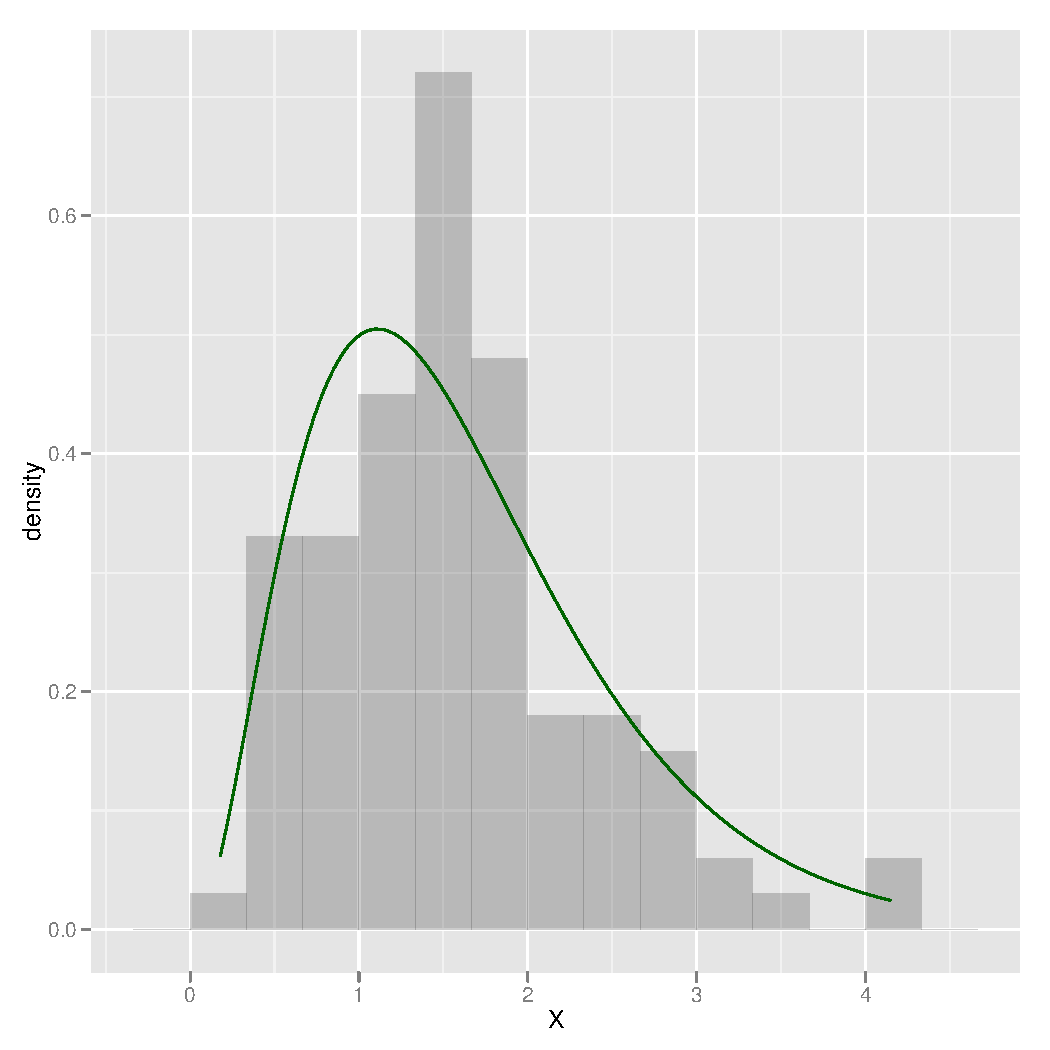
\includegraphics[width=0.8\textwidth]{figure/plots} 
\end{knitrout}

\caption{Histogram of $n = 100$ iid samples from $\Gamma$($r$=3.13, $\lambda$=1.92) with density overlayed.}
\end{figure}

While it's clear that my histogram resembles the density of our sample distribution (though, it could stand to resemble it more closely), I'm remiss to say my estimators are not very close to their targets\ldots. 

\item[d)]



The mean our 1000 estimations of $r$ and $\lambda$ are 3.2619 and 2.0066, respectively. The SD of our the 1000 estimations is 0.5382 and 0.349.  

\begin{figure}[ht!]
\centering
\begin{knitrout}
\definecolor{shadecolor}{rgb}{0.969, 0.969, 0.969}\color{fgcolor}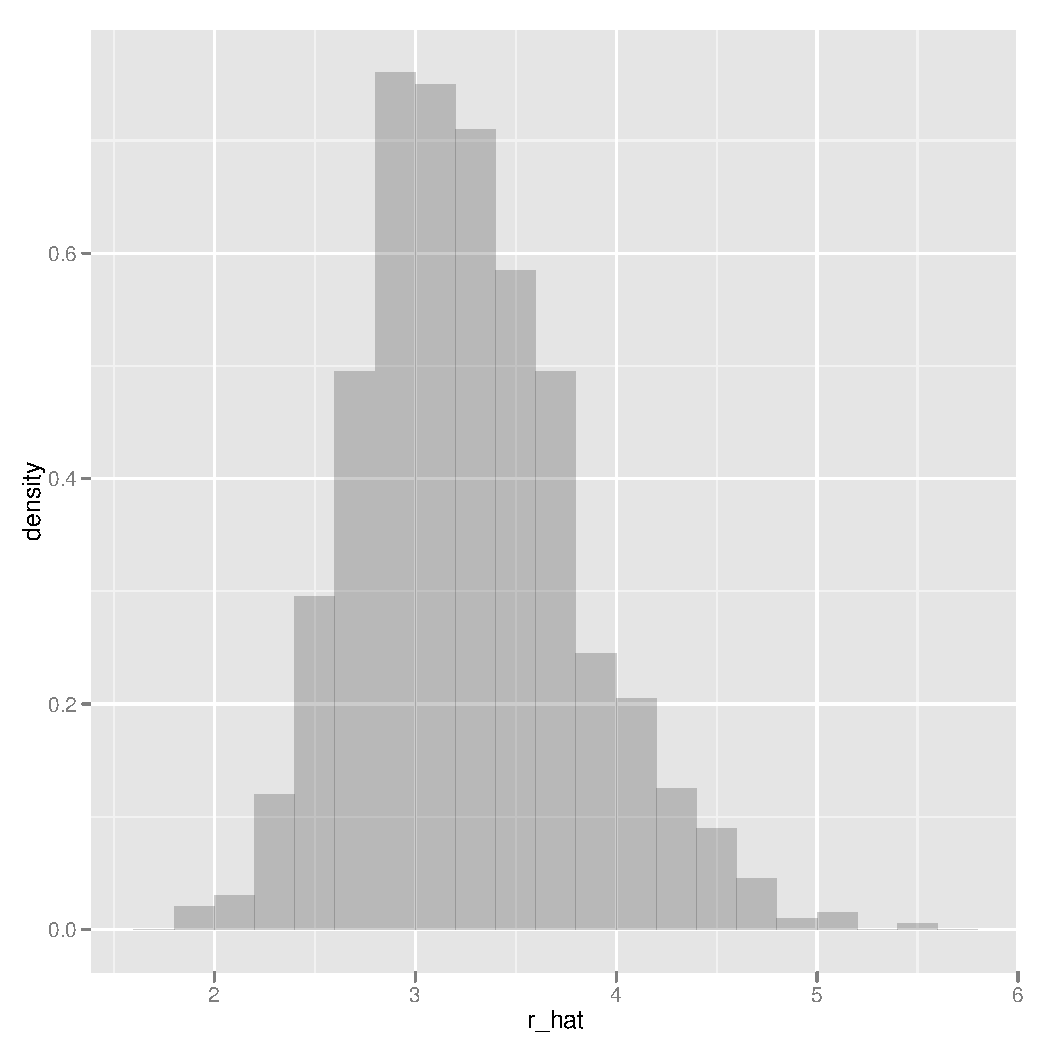
\includegraphics[width=0.65\textwidth]{figure/partDPlots} 
\end{knitrout}

\begin{knitrout}
\definecolor{shadecolor}{rgb}{0.969, 0.969, 0.969}\color{fgcolor}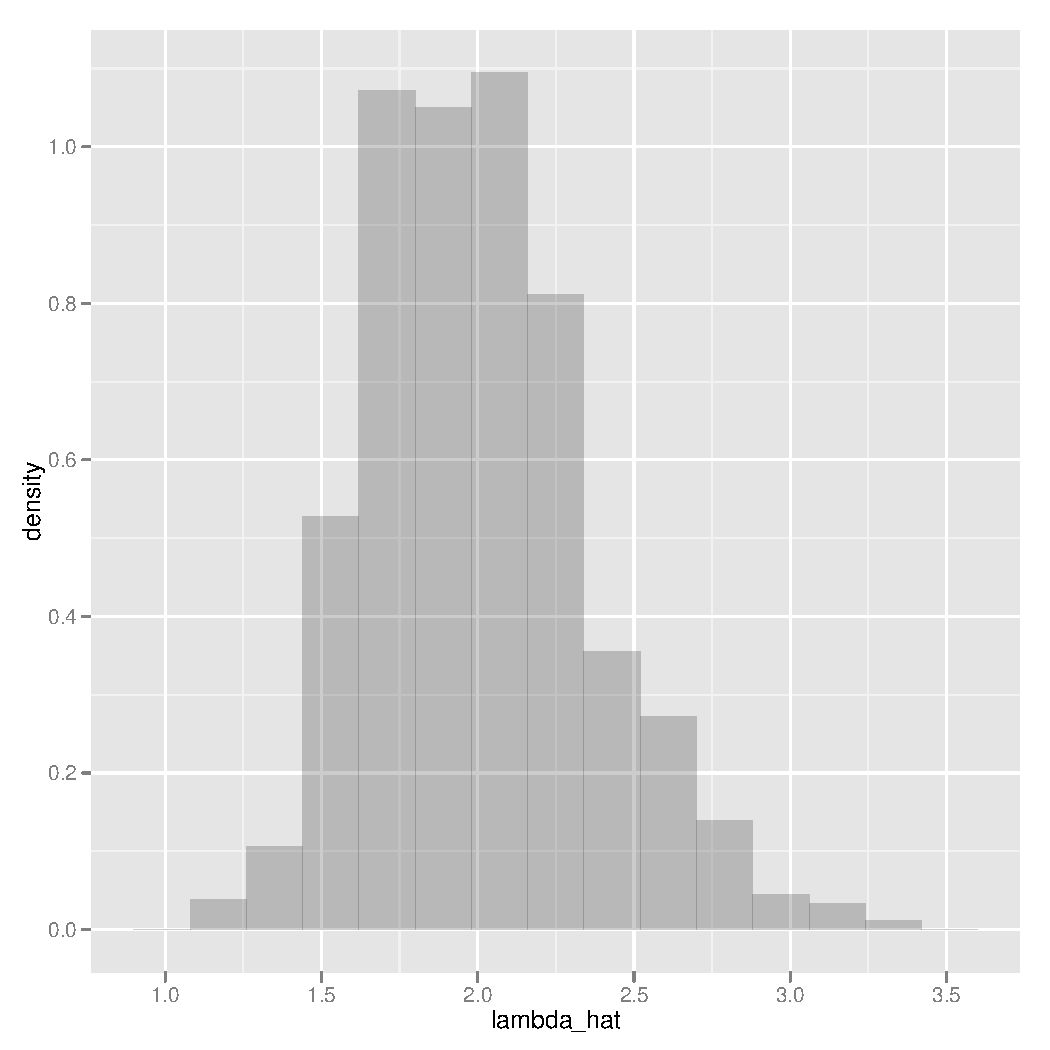
\includegraphics[width=0.65\textwidth]{figure/partDPlots2} 
\end{knitrout}

\caption{Histograms for $\hat{r}$ and $\hat{\lambda}$ when $n=100$}
\end{figure}
\end{enumerate}

\paragraph{\#9.}




The mean our \textit{new} 1000 estimations of $r$ and $\lambda$ are 3.1447 and 1.9287, respectively. The SD of our the 1000 estimations is 0.1654 and 0.1062. It seems that our estimators are, indeed, converging to their targets. I'm willing to say this is most likely a consequence of the fact that $\hat{\mu}_{k} \to E(X^k)$ with whatever speed the weak-law of large numbers affords us.

\begin{figure}[ht!]
\centering
\begin{knitrout}
\definecolor{shadecolor}{rgb}{0.969, 0.969, 0.969}\color{fgcolor}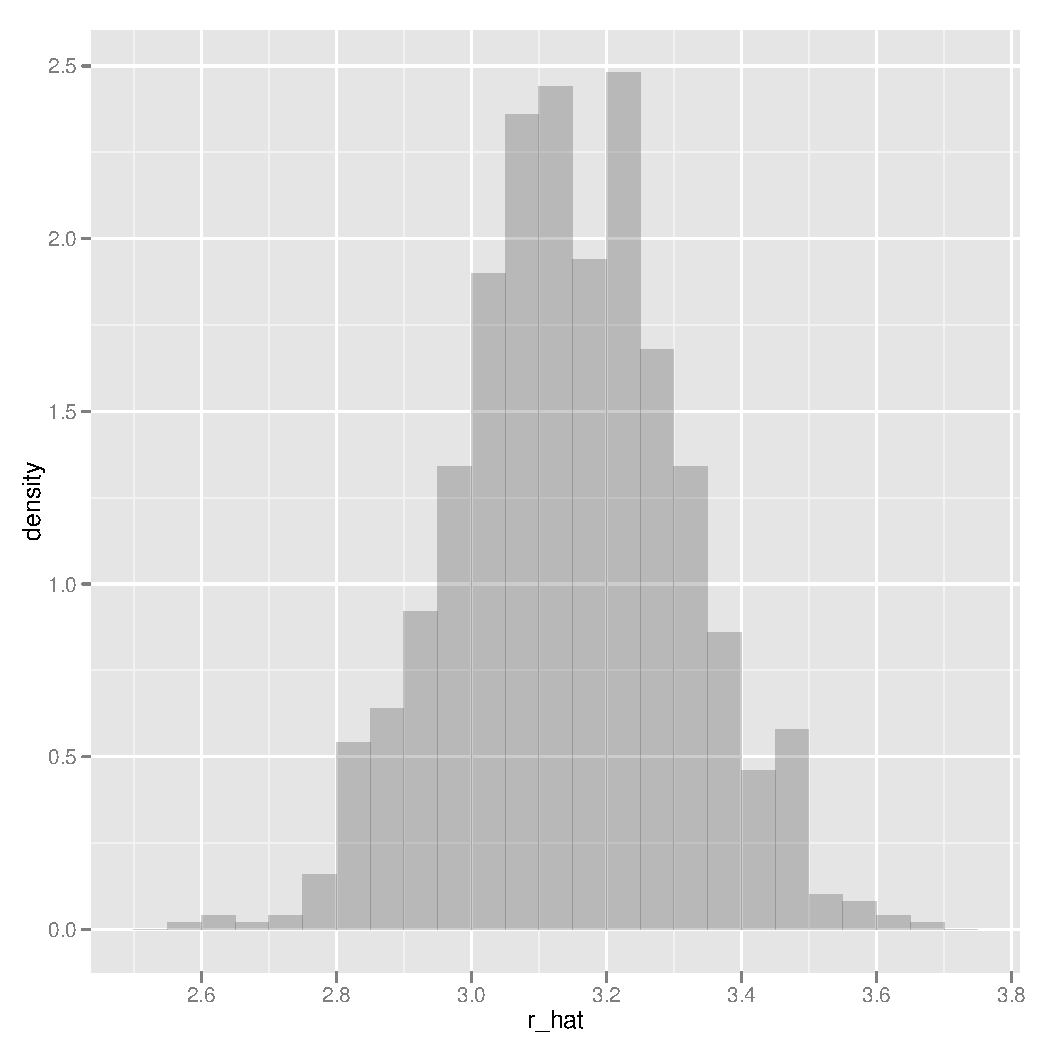
\includegraphics[width=0.65\textwidth]{figure/prob9Plots} 
\end{knitrout}

\begin{knitrout}
\definecolor{shadecolor}{rgb}{0.969, 0.969, 0.969}\color{fgcolor}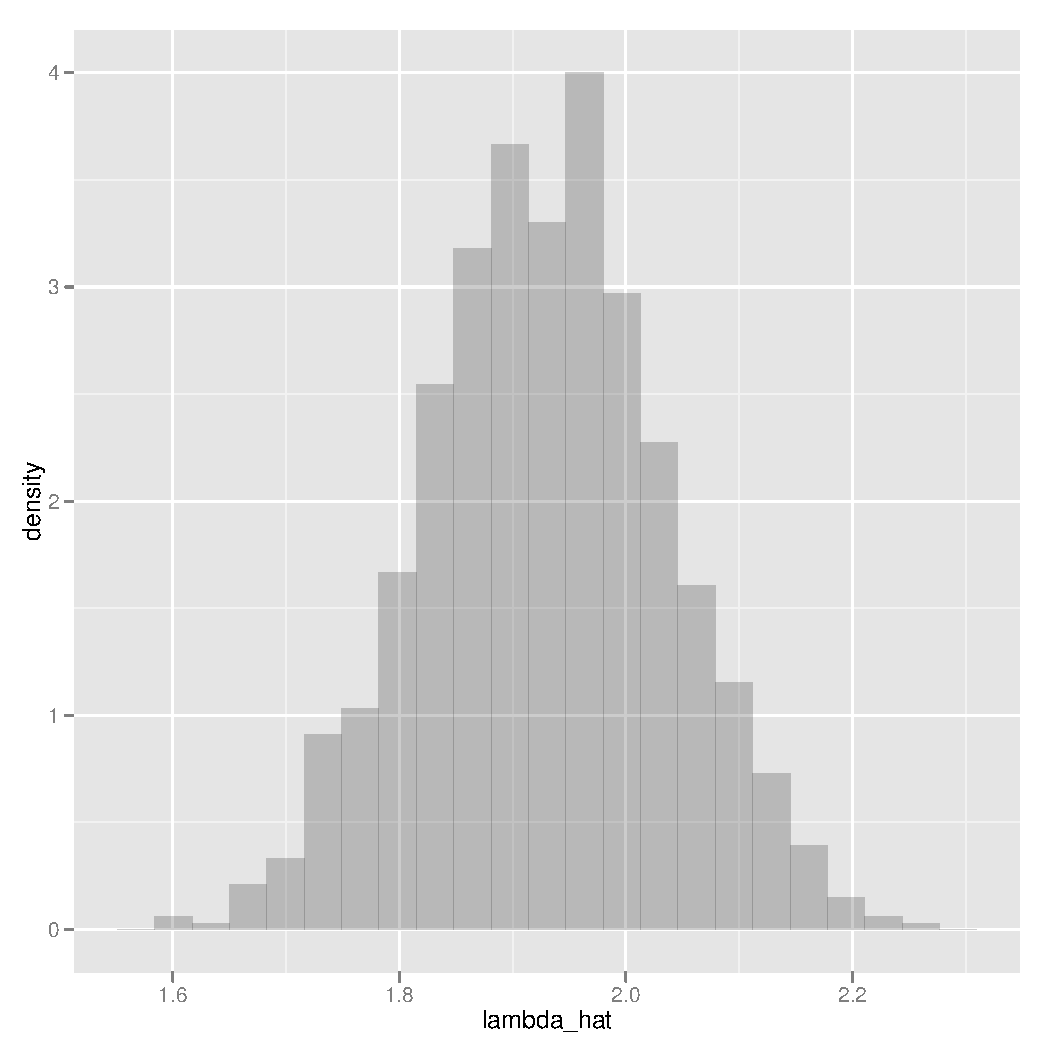
\includegraphics[width=0.65\textwidth]{figure/prob9Plots2} 
\end{knitrout}

\caption{Histograms for $\hat{r}$ and $\hat{\lambda}$ when $n=1000$}
\end{figure}


\end{document}
